\documentclass[12 pt]{article}

% Useful example: http://www.bibtex.org/Using/

\usepackage[margin=1 in]{geometry}

\usepackage{cite}
\usepackage{natbib}
\usepackage{graphicx}
\usepackage{float}

\usepackage{hyperref}
\hypersetup{
    colorlinks=true,
    linkcolor=blue,
    filecolor=magenta,      
    urlcolor=cyan,
}

% SOURCE FOR COMMAND BELOW: https://tex.stackexchange.com/questions/30720/footnote-without-a-marker
\newcommand\blfootnote[1]{%
  \begingroup
  \renewcommand\thefootnote{}\footnote{#1}%
  \addtocounter{footnote}{-1}%
  \endgroup
}

\title{Data Mining\\Assignment 1\\Bonus Mark Documentation\\(CPSC473)}
\author{Galen Michael Seilis \\}
\date{October 23, 2020}

\begin{document}
\maketitle
\pagebreak

\section{Introduction}
The purpose of this report is to explain what I've attempted in improving the Apriori algorithm. There are numerous proposed improvements to the Apriori frequent pattern mining algorithm.\cite{Park1995, Gu2011, AlMaolegi2014, Yuan2017, Liu2017}

\section{apriori: Self-Joining}

In a sense my \textbf{apriori.py} script is an improvement because it uses a filtered self-join of the frequent patterns from the last iteration for the candidate patterns of the current iteration. This is certainly an improvement over checking all combinations of items with length $k$ for the $k$th iteration of the algorithm. I did not implement this slower version of the Apriori algorithm, but I suppose my implementation is already not the slowest because it does not explore the entire powerset of the itemset.\footnote{The size of the powerset is an exponential function of the size of the itemset.}

\section{rmtid: Removing Useless Transactions}

The first approach I tried in order to improve the Apriori algorithm was to keep track of only the transactions that may have relevant information. Doing so would save me from having to loop over every single transaction. So, if I had the $i$th transaction $t_i$ from the transaction database, and found that \textit{none} of the candidates from $C_k$ were subsets of $t_i$ then I know that I would never need to consider that transaction again in further iterations of the algorithm. This is in part because the downward closure property tells us that if none of the current candidates were in a transaction, then none of the future candidates will be either.\\

It is natural in Python to simply loop over the lines of a file, but since I wanted to avoid this looping I had to devise another way. What I needed was some way to read specific transactions from the database file, and in any order.\footnote{In a sense, what I was going for was \textit{random access} to the database.} To do this I would need to know where the transactions each start and stop in the file, so I knew I had to loop over the file at least once. I accomplished this by modifying the first scan of the database file so that it would construct a Python dictionary of where each transaction started and stopped. Next I coded a function that when given the start and stop indices of a transaction, would read it directly from the database file.\footnote{I used Python's seek and read methods to write this function.}\\

With this functionality of reading specific transactions, I also had that dictionary of the transaction ID's with their start and stops. To remove a transaction from future iterations of the apriori algorithm was a simple matter of unreserving those entries from memory.\footnote{You can do this with a Python dictionary by simply using \textbf{del dict[key]}.} As I looped over the transactions, I would compare them to each candidate. If a transaction was not a proper/improper superset of any of the candidates, then it was deleted from the dictionary.\\

While this approach doesn't keep the transaction itemsets themselves, it is true that a tradeoff of this approach is the use of more memory to keep track of which transactions are useful. As this method is fundamentally similar to the AprioriTID algorithm that also keeps track of transactions, as Park et al 1995 explains, I expect rmtid to be less efficient than apriori for smaller databases but become more efficient than apriori for large databases.\cite{Park1995}

\section{p\_rmtid: Parallelization with Removal of Useless Transactions}

Having completed the rmtid implementation of the apriori algorithm that keeps track of transactions, and deletes the ones from memory that are no longer useful, I realized that I had made scanning each transaction something that can be done independently. If I can scan each transaction independently of each other, then I could parallelize this process. That is exactly what p\_rmtid does that is different from rmtid, but is otherwise identical in every respect. That is, p\_rmtid takes the current collection of transactions and divides them into a number of batches equal to the number of available CPUs, and does the database scan on these batches separately. Once these scans are complete for the current iteration, the counts are pooled so that the minimum support threshold can be applied to the patterns.

\section{Comparitive Analysis}

In this section I will briefly summarize the results of some performance testing I did on my implementations of the apriori algorithm. In order to make some general comparisons, I ran each algorithm multiple times on each provided test data file with different minimum support thresholds depending on run times. Since choice of minimum support threshold changes the run time of the algorithms, and I could not run \textit{connect.txt} as low as the others, I've only chosen specific minimum support thresholds to report on.\footnote{See \textit{performance\_results.csv} for all the performance test data I recorded.} This subset of the results is summarized in Table \ref{tab:marginal}. Among these results, I would say that neither \textbf{rmtid\_ariori.py} nor \textbf{p\_rmtid\_ariori.py} were a general improvement over \textbf{ariori.py}. In fact, \textbf{rmtid\_ariori.py} was always slower despite the rational behind. However, \textbf{p\_rmtid\_ariori.py} was sometimes faster with the strongest example being on the \textit{connect.txt} dataset. My hypothesis about this is that there are overhead costs to my attempted improvements that sometimes pay off. As you'll see in a later section of this report, graph analysis gives some hints as to the properties that make \textit{connect.txt} different from the other transaction database files.

\begin{table}[H]
\caption{Pivot table aggregating the mean and standard deviation of the runtimes of the different implmentations grouped by transaction database file.}
\centering
\begin{tabular}{llrrr}
\hline
data\_file & program &    mean run time (s) &    std run time (s) & min sup \\
\hline
1k5L.txt & apriori.py &  2.102962 &  0.464741 & 0.01 \\
         & p\_rmtid\_apriori.py &  1.730705 &  0.142890 & 0.01 \\
         & rmtid\_apriori.py &  2.320507 &  0.493646 & 0.01 \\
connect.txt & apriori.py &  2338.118468 &   77.472895 & 0.9 \\
            & p\_rmtid\_apriori.py &   996.285629 &   45.446046 & 0.9 \\
            & rmtid\_apriori.py &  2553.477626 &  216.182645 & 0.9 \\
data.txt & apriori.py &  0.044466 &  0.006801  & 0.01 \\
         & p\_rmtid\_apriori.py &  0.417181 &  0.017041  & 0.01 \\
         & rmtid\_apriori.py &  0.042302 &  0.003749  & 0.01 \\
retail.txt & apriori.py &   85.145460 &  1.740205  & 0.01 \\
           & p\_rmtid\_apriori.py &   87.852953 &  2.080159  & 0.01 \\
           & rmtid\_apriori.py &  101.006186 &  1.363830  & 0.01 \\
t25i10d10k.txt & apriori.py &  208.863822 &  6.460889  & 0.01 \\
               & p\_rmtid\_apriori.py &  121.212862 &  1.544932  & 0.01 \\
               & rmtid\_apriori.py &  207.789247 &  1.602973  & 0.01 \\
\hline
\end{tabular}
\label{tab:marginal}
\end{table}

While Table \ref{tab:marginal} gives a slice of the data I collected on the relative performance, I decided to make some visualizations to show how the different algorithms' performance changes with the minimum support threshold on each transaction database file. As you can see from Figure \ref{fig:mtrt}, my attempted improvements were not better in most cases. However, as hinted by Table \ref{tab:marginal}, sometimes \textbf{p\_rmtid\_ariori.py} was faster. You can see this conditional improvement in the traces associated with \textit{connect.txt}, but the trend is also supported by \textit{t25i10d10k.txt}. The is a section of the plot for \textit{retail.txt} where the run times become erratic between the minimum support thresholds of 0.5 and 0.8, and this was unfortunately due to other programs I was running that were using enough resources to distrupt these performance tests.\footnote{Whoops!}

\begin{figure}[H]
	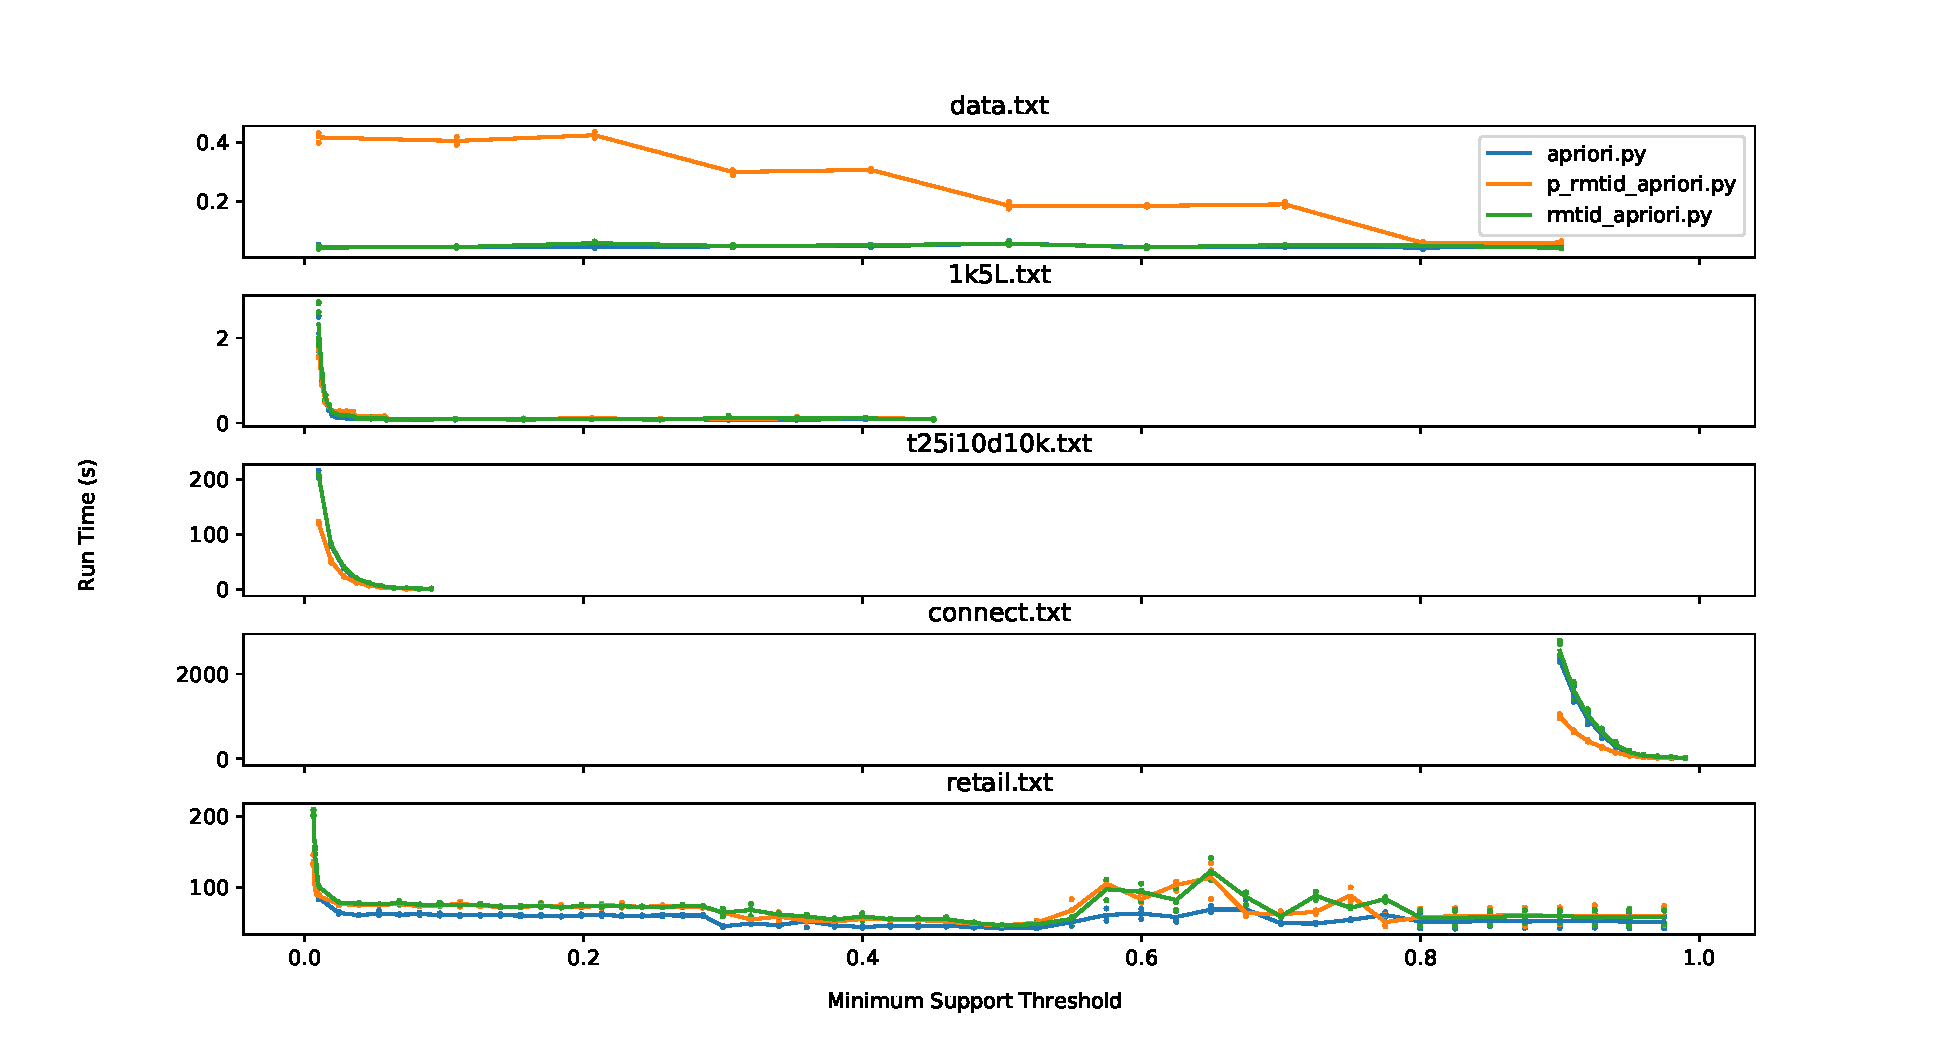
\includegraphics[scale=0.5]{minsup_stats}
	\caption{Comparison of three scripts performing frequent pattern mining. The vertical axes of each subplot are the run time of the algorithm, and the horizontal axis is the minimum support threshold that the algorithm was run at. Each subplot is titled by the transaction database file that the algorithms were run on, and the colour legend indicates which colour corresponds to which script. The scatter points are actual data points, and the lines are drawn between the mean runtime at a given minimum support threshold.}
	\label{fig:mtrt}
\end{figure}

\section{Graph Analysis}
\label{section:graph}

I was trying to explain to myself why \textit{connect.txt} which contains 67557 transaction took a lot longer to mine frequent patterns from than \textit{retail.txt}, which has 88162 transactions. To emphasize this difference in perfomance, my vanilla Apriori implementation completed the frequent pattern mining for \textit{retail.txt} at a minimum support threshold of 0.5 in a few seconds short of a minute and found a single frequent pattern, while those same conditions on \textit{connect.txt} took 2 days, 5 hours, 31 minutes, and 52 seconds to find 992813 frequent patterns and had not completed execution! I concluded that something must explain this orders-of-magnitude difference in time completion.\\

\begin{figure}[H]
	\centering
	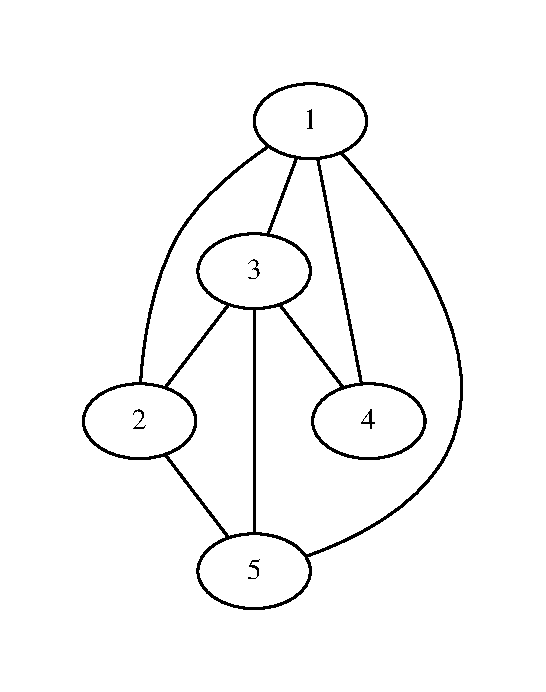
\includegraphics[scale=0.7]{single_example}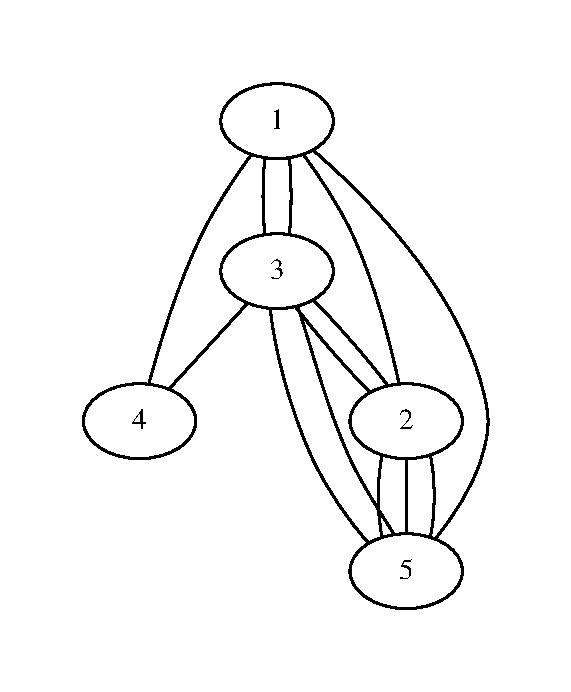
\includegraphics[scale=0.7]{multi_example}
	\caption{(left) A simple graph of the items in \textit{data.txt} such that they share an edge whenever they share a transaction. (right) A multigraph of the items in \textit{data.txt} such that they share an edge \textbf{for every} instance that they share a transaction.}
	\label{fig:graphs}
\end{figure}

I chose to examine this from a graph theory perspective by encoding the transactions into graphs or multigraphs and considering their graph properties. For the graph representation, I consider the vertices to be items and the edges between the items to be the relation of the items sharing at least one transaction.\footnote{By \textit{sharing a transaction} between vertices $n_i$ and $n_j$, I mean there exists an edge $(n_i, n_j)$ if there exists a transaction such that $\lbrace n_i, n_j \rbrace$ is one of its subsets.} I similarly constructed a multigraph representation, however the vertices have multiple edges reflecting that a pair of items may share multiple transactions. Figure \ref{fig:graphs} shows these graph representations for the transactions in \textit{data.txt}, but I did not include these diagrams for the other graphs as they were uninterpretable and computationally slow to create.\\

Once I had created the graph representations described above, I decided to calculate some of the basic properties of these graphs which are given in Table \ref{tab:graphs}. I did not find the number of transactions surprising, however it was very surprising that the number of items in \textit{connect.txt} was only 129 given the number of transactions. The graph density is somewhat indicative the difficulty of a database, but not entirely because it does not account for the size of the database. For example, \textit{data.txt} and \textit{connect.txt} have similar densities but the latter clearly takes a lot longer to process. What starts to become more telling is the number of edges and the average degree of the multigraph representations of the databases. Consider that \textit{connect.txt} was considerably more difficult to process, and it also has considerably more edges and a higher average degree than any of the other databases.

\begin{table}[H]
\caption{Summary of the properties of each graph representation of each testing dataset.}
\centering
\begin{tabular}{lccccc}
	\hline
	Dataset & \# Transactions & \# Vertices & \# Edges & Average Degree & Graph Density \\
	\hline
	data.txt & 4 & 5 & 13 & 5.2 & 0.8 \\
	1k5L.txt & 1000 & 825 & 17900 & 43.39 & 0.045 \\
	t25i10d10k.txt & 9976 & 929 & 3223585 & 6939.90 & 0.73 \\
	retail.txt & 88162 & 16407 & 7164335 & 873.33 & 0.027 \\
	connect.txt & 67557 & 129 & 61003971 & 945798 & 0.83 \\
	\hline
\end{tabular}

{\tiny The number of edges and the average degree are from the multigraph representation. The graph density is from the simple graph representation.}
\label{tab:graphs}
\end{table}

These graph representations seem to give an intuition as to why some transaction databases will be more difficult to process in a way that is not simply explained by the number of items or transactions. There is abstractly a notion of 'connectedness' between transactions through shared items that make them more difficult to process. At a given support threshold, more of this connectedness will imply that more of the candidate itemsets will pass that threshold, thus leading to even more of the larger candidate sets to be considered.

\section{Future Considerations}

In every open-ended project there are unresolved thoughts and tasks, and this project to implement an improved Apriori algorithm is not different in this respect. This section will briefly discuss some of those unresolved thoughts on what I might do differently in the future.\\

The first topic left unresolved is just looking at tweaking my implementation of the original Apriori algorithm. There may be different type casting choices I could try, or perhaps there are different loop or comprehension structures that I could have tried. For example, I noticed when I profiled \textbf{apriori.py} that most of the time was spent on repeatedly performing the same list comprehension in order to clean lines from the transaction database. Perhaps this could be improved. There are also some dummy variables in my code that were included with the anticipation of their eventual use, but in the end I am not using them. It would be a minor improvement to remove them.\\

You'll see from my source files that there are functions that are common to all the scripts, and that perhaps some of them could have been factored and/or placed in a separate 'utilities' file just so the scripts are more concise.\\

While I took the time to profile and carefully think about \textbf{apriori.py}, I cannot say I did the same for \textbf{rmtid\_apriori.py} or \textbf{p\_rmtid\_apriori.py}. The latter two were coded in a \textit{stream-of-consciousness} fashion where I simply used the data types, data structures, loops, and comprehensions that most easily came to mind at the time instead of planning and reflecting on them. Perhaps going back to carefully interpret profiling results of these scripts would show me inefficiencies that could be readily improved.\\

While the whole point of \textbf{p\_rmtid\_apriori.py} was to use parallelization to improve performance, I only did it for scanning the database transactions. I am confident looking through my code that there were other opportunities to easily include more parallel structures. For example, the selection of frequent patterns that met the minimum support threshold should be parallelizable because whether one candidate was frequent enough at a given iteration will not strictly depend on whether another is frequent enough in the same iteration.\footnote{Note that I am carefully not contradicting the downward closure property here.}\\

Lastly, as I pointed out in the introduction, there are other proposed improvements on the Apriori algorithm. Perhaps some combination of them could yield even better performance.

\pagebreak

\bibliography{citations}{}
\bibliographystyle{unsrt} % https://stackoverflow.com/questions/144639/how-to-order-citations-by-appearance-using-bibtex
\end{document} 
